\documentclass[12pt]{article}
\usepackage[margin=2.5cm]{geometry}
\usepackage{enumerate}
\usepackage{amsfonts}
\usepackage{amsmath}
\usepackage{fancyhdr}
\usepackage{amsmath}
\usepackage{amssymb}
\usepackage{amsthm}
\usepackage{mdframed}
\usepackage{graphicx}
\usepackage{subcaption}
\usepackage{adjustbox}
\usepackage{listings}
\usepackage{xcolor}
\usepackage{courier}
\usepackage[utf]{kotex}
\usepackage{hyperref}

\definecolor{codegreen}{rgb}{0,0.6,0}
\definecolor{codegray}{rgb}{0.5,0.5,0.5}
\definecolor{codepurple}{rgb}{0.58,0,0.82}
\definecolor{backcolour}{rgb}{0.95,0.95,0.92}

\lstdefinestyle{mystyle}{
    backgroundcolor=\color{backcolour},
    commentstyle=\color{codegreen},
    keywordstyle=\color{magenta},
    numberstyle=\tiny\color{codegray},
    stringstyle=\color{codepurple},
    basicstyle=\ttfamily\footnotesize,
    breakatwhitespace=false,
    breaklines=true,
    captionpos=b,
    keepspaces=true,
    numbers=left,
    numbersep=5pt,
    showspaces=false,
    showstringspaces=false,
    showtabs=false,
    tabsize=1
}

\lstset{style=mystyle}

\pagestyle{fancy}
\renewcommand{\headrulewidth}{0.4pt}
\lhead{CSC 369}
\rhead{Worksheet 8 Solution}

\begin{document}
\title{CSC 369 Worksheet 8 Solution}

\maketitle

\bigskip

\begin{enumerate}[1.]
    \item

    \bigskip

    I need to translate the addresses in the following sets of parameters

    \begin{itemize}
        \item \texttt{./segmentation.py -a 128 -p 512 -b 0 -l 20 -B 512 -L 20 -s 0}
        \item \texttt{./segmentation.py -a 128 -p 512 -b 0 -l 20 -B 512 -L 20 -s 1}
        \item \texttt{./segmentation.py -a 128 -p 512 -b 0 -l 20 -B 512 -L 20 -s 2}
    \end{itemize}

    \bigskip

    Running each command results as follows, with the following sets of valid and invalid
    addresses

    \bigskip

    \begin{itemize}
        \item \texttt{./segmentation.py -a 128 -p 512 -b 0 -l 20 -B 512 -L 20 -s 0}

        \begin{center}
        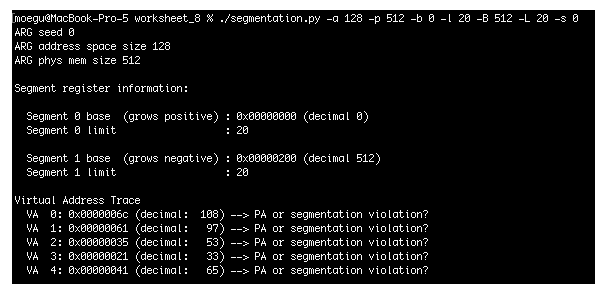
\includegraphics[width=0.8\linewidth]{images/worksheet_8_solution_3.png}
        \end{center}

        \begin{itemize}
            \item \texttt{VA  0: 0x0000006c (decimal:  108)} $\to$ Segment violation
            \item \texttt{VA  1: 0x00000061 (decimal:   97)} $\to$ Segment violation
            \item \texttt{VA  2: 0x00000035 (decimal:   53)} $\to$ Segment violation
            \item \texttt{VA  3: 0x00000021 (decimal:   33)} $\to$ Segment violation
            \item \texttt{VA  4: 0x00000041 (decimal:   65)} $\to$ Segment violation
        \end{itemize}

        \item \texttt{./segmentation.py -a 128 -p 512 -b 0 -l 20 -B 512 -L 20 -s 1}
        \item \texttt{./segmentation.py -a 128 -p 512 -b 0 -l 20 -B 512 -L 20 -s 2}
    \end{itemize}


    \bigskip

    \underline{\textbf{Notes}}

    \begin{itemize}
        \item I need help on this question
        \item How do we know tell which VA goes to which segmentation?
        \item How could VA 0 (decimal 108) be valid at SEG 1 (decimal 492) when limit is 20?
        \item \textbf{Segmentation}

        \begin{itemize}
            \item \textbf{Segment} is a contigous portion of the address space of a particular length
            \item Is about the big chunk of space in the middle

            \begin{center}
            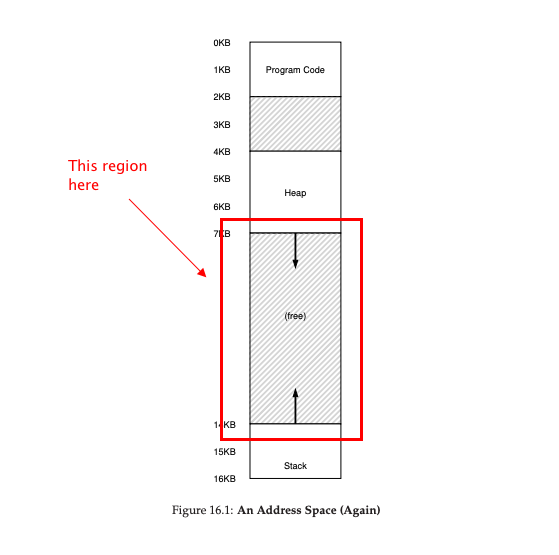
\includegraphics[width=0.7\linewidth]{images/worksheet_8_solution_1.png}
            \end{center}

            \item \textbf{Segmentation} allows the OS to place each one of the logical segments (i.e. stack, heap, program code)
            in different parts of physical memory, and avoid filling physical memory with unused virtual address space


            \begin{center}
            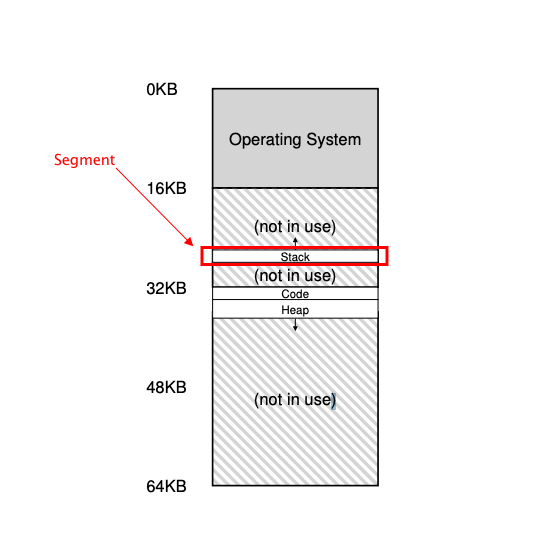
\includegraphics[width=0.7\linewidth]{images/worksheet_8_solution_2.png}
            \end{center}
        \end{itemize}

        \item \textbf{Which Segment Are We Referring To?}

        \begin{itemize}
            \item \textbf{Explicit Approach}

            \begin{itemize}
                \item Chops up address space into segments based on top few bits of the virtual address
            \end{itemize}

            \begin{center}
            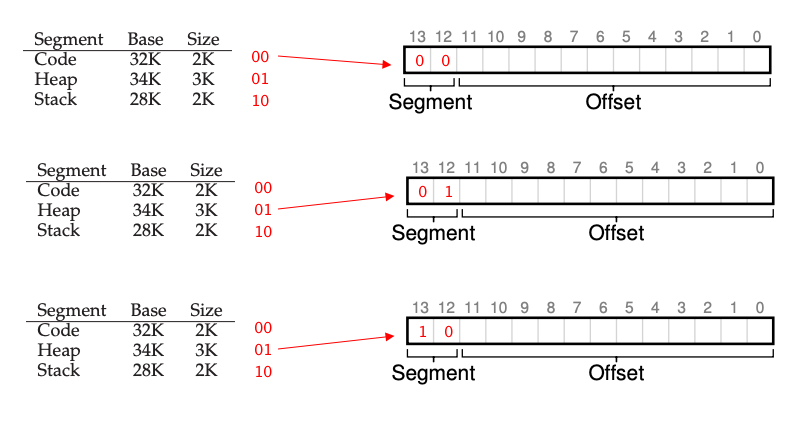
\includegraphics[width=\linewidth]{images/worksheet_8_solution_4.png}
            \end{center}
            \item \textbf{Implicit Approach}
        \end{itemize}
    \end{itemize}


\end{enumerate}

\end{document}